\section{Déroulement du travail}

% Un titre de section aussi long est \textbf{fortement déconseillé} mais j'ai configuré le header pour qu'il le gère.

\subsection{Description de la mission}
\subsubsection{Le site web Répertoire Vert}

Ma mission concernait le site web du projet Répertoire Vert.
\\\\
Le Répertoire Vert est un outil de référencement et d’évaluation des produits et services verts proposés dans un rayon de 130 km autour d’un point de référence (ici Genève). 
Il permettra au «consomm’acteur» de trouver le meilleur produit/service «vert» en toute confiance et à un prix raisonnable, 
et à l’entreprise proposant un produit/service, d’avoir une meilleure visibilité, une reconnaissance active, et de vendre davantage.
\\\\

Le répertoire vert propose une répartition de l’activité économique « verte » en 28
secteurs principaux, comme Alimentation et Boisson, Green Building ou encore Santé et Bien-être.
\\\\
Il détermine 4 niveaux de référencement basés sur une triple évaluation :\\
• Celle de l’association gaea21\\
• Celle des professionnels de la branche d’activité concernée\\
• Celle du public (les consomm’acteurs)\\
\\
Ainsi, les entreprises peuvent se démarquer des produits « pseudo-verts » mis en vente sur le marché de manière abondante, et par conséquent, donner confiance , orienter et informer le consom’acteur de manière éthique.
Ce projet se décline en un site web et une application mobile.
\\\\

\begin{figure}[H]
    \centering
    
\includegraphics[width=8cm]{logo_repertoire_vert.png}
    \caption{Logo du Répertoire Vert}
\end{figure}

Le site s'adresse donc aux entreprises proposant des produits et/ou services verts, aux particuliers souhaitant trouver ces produits et services, 
mais aussi aux villes/régions qui peuvent voir les entreprises vertes disponibles sur leur territoire. Il se compose donc de 3 parties distinctes, 1 pour chaque cible.
Je me suis occupée principalement de la partie dédiée aux entreprises.
\\\\
\begin{figure}[H]
    \centering
    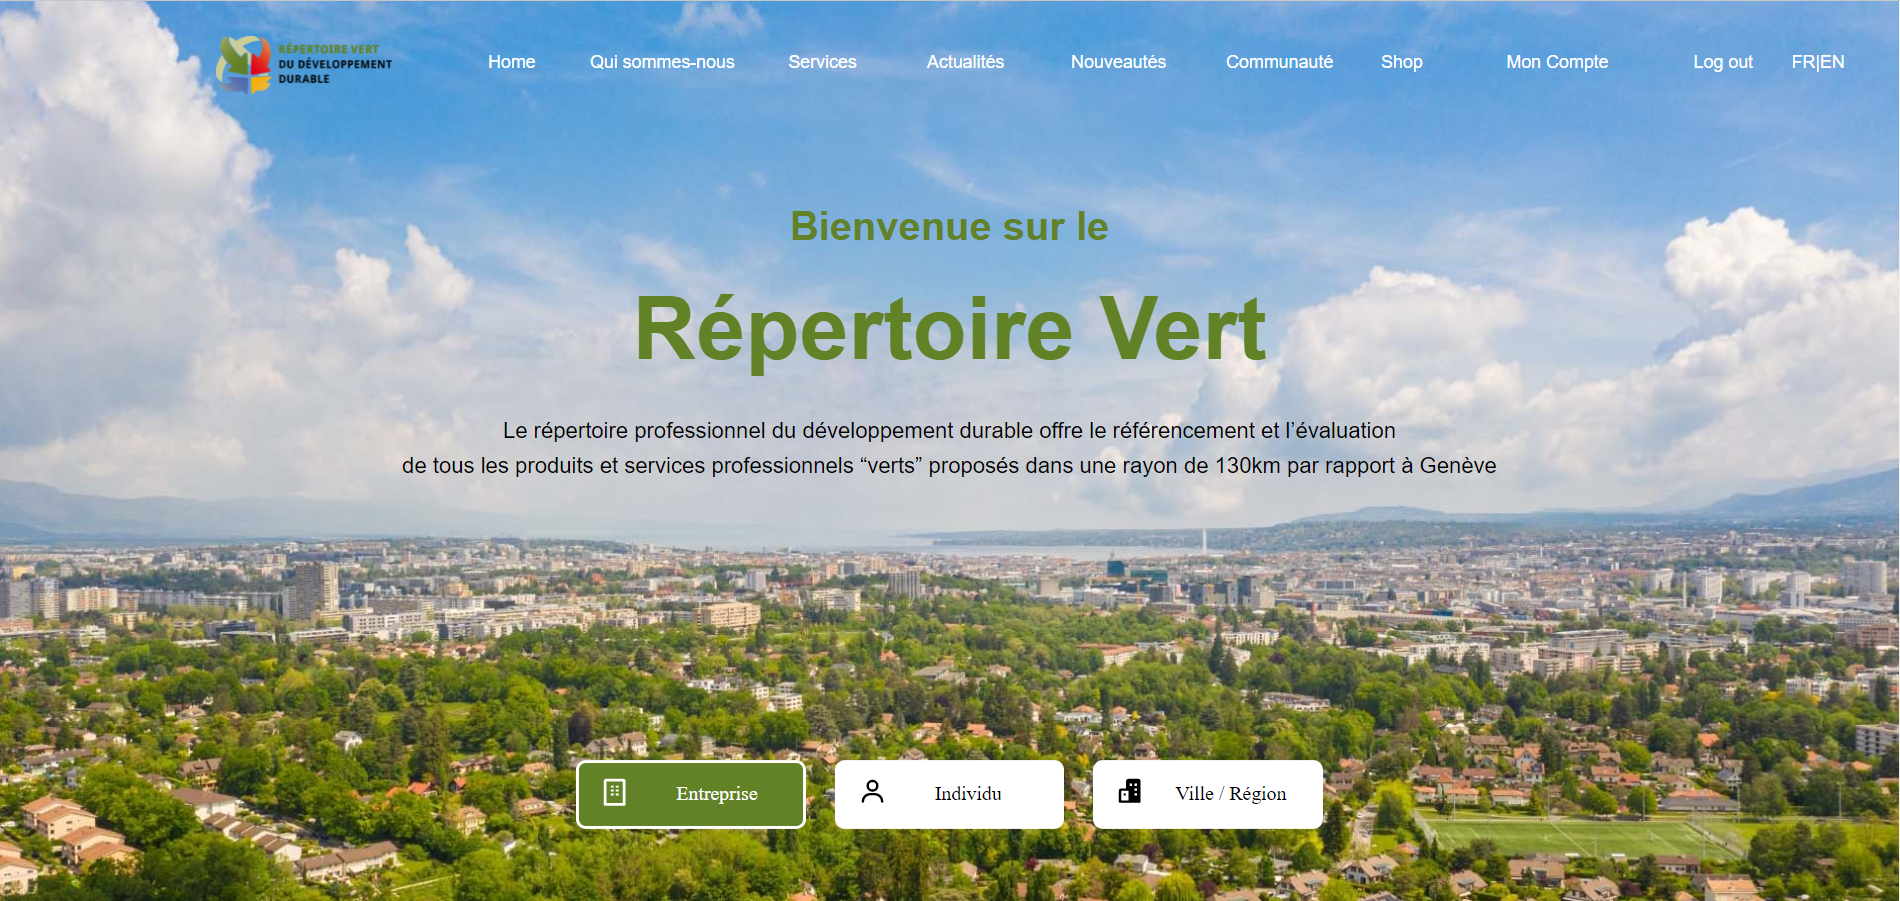
\includegraphics[width=\textwidth]{homepage_entreprise.png}
    \caption{Page d'accueil entreprise}
\end{figure}


Sur le site, une entreprise doit pouvoir se connecter, ajouter des produits et/ou services, visualiser son profil et ses statistiques.
Plus largement, on pourra visualiser l'ensemble des entreprises inscrites dans la région, mais également en fonction des secteurs d'activité. Le site devra aussi être un site e-commerce permettant d'acheter des produits et services verts.

\subsubsection{Fonctionnalités à réaliser}

Les tâches à réaliser se définissaient petit à petit. En effet il est important dans l'association de savoir prendre des initiatives : 
on nous donne les instructions dans les grandes lignes, à nous de voir précisément les différentes tâches à réaliser pour atteindre l'objectif posé.
\\\\
Au niveau des fonctionnalités donc, je devais dans un premier temps m'occuper de la représentation des entreprises sur des cartes. 

La 1ère devait figurer sur le profil de l'entreprise avec un point la représentant sur cette carte.

La 2nde devait être plus générale en affichant toutes les entreprises inscrites sur le Répertoire vert. 
Elle devait faire l'objet d'un filtre comportant plusieurs critères pour les entreprises : catégorie, sous-catégorie, code postal, prix des produits/services vendus, etc\dots
\\\\
Mais d'autres tâches se sont peu après avérées beaucoup plus urgentes que la carte des entreprises. J'ai donc dû me charger de rendre l'inscription, la connexion et la réinitialisation de mot de passe fonctionnelles, 
mais aussi de faire en sorte que l'utilisateur puisse visualiser et gérer entièrement son profil et ses produits/services. J'ai aussi travaillé sur le responsive du site et sur la création de diverses nouvelles pages.

\subsubsection{Gestion de projet}

Outre le développement web, mon autre rôle majeur était celui de chef de projet du Répertoire Vert, se constituant d'une équipe de 3 à 4 autres développeurs.
J'étais donc responsable du travail de mon équipe et devait m'assurer du respect des deadlines. Pour cela, il était parfois nécessaire de remplir des documents tels qu'un poker planning afin d'évaluer la difficulté des tâches et ainsi prévoir la durée de leur réalisation.
\begin{figure}[H]
    \centering
    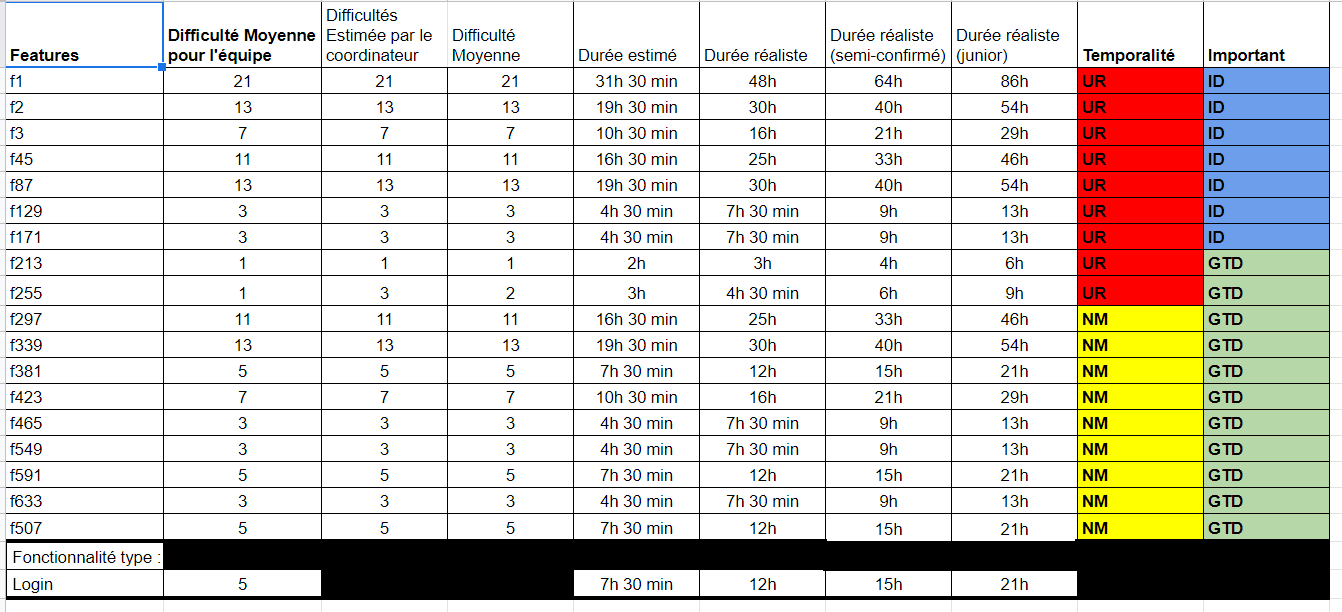
\includegraphics[width=\textwidth]{poker planning.png}
    \caption{Planning Poker}
\end{figure}

Être chef de projet impliquait aussi d'accueillir les nouveaux arrivants, en leur apportant toute l'aide dont ils ont besoin pour prendre en main le projet, notamment expliquer où se trouvent les différents fichiers, la méthodologie à adopter, ou encore les commandes utiles en invite de commandes. J'ai eu l'occasion d'accueillir 5 nouvelles recrues.
\\Mais même de manière plus générale, j'aidais souvent les membres de mon équipe dans leur tâche, ce qui m'a permis d'étudier des fonctionnalités sur lesquelles je n'étais normalement pas censée travailler.
\\\\
Tout cela m'a permis d'acquérir une vision globale du projet, me permettant de cerner les différentes tâches restantes et comment elles devaient être réalisées.
\\\\
Une autre responsabilité que j'avais était la mise en production du site web deux fois par semaine. 
\\Pour ce faire, il fallait mettre à jour le site sur un serveur Linux distant à l'aide de Git, un logiciel de gestion de versions que j'ai particulièrement utilisé durant ce stage. Cette étape de mise en production était très importante, car elle nous permettait d'appréhender d'éventuels bugs tout de suite plutôt que de les accumuler, ce qui assurait la qualité du rendu.


\pagebreak
\subsection{Antécédents}
Défi : se familiariser avec le code existant et les nombreux fichiers. Certaines fonctionnalités étaient déjà créées et pouvaient donc être réutilisés
\pagebreak
\subsection{Méthode choisie et objectifs visés}
Objectifs V0
suivi du travail


\pagebreak
\subsection{Planning prévisionnel du travail}
\pagebreak
\subsection{Application de la méthode}

Fonctionnalités en détail
Problèmes rencontrés
Git
Communication avec autres départements

\pagebreak
\subsection{Résultats par rapport à l'objectif et planning réel}
Compétences acquises

% Une version humainement lisible d'une fork bombe peut s'écrire ainsi:
% % Il ny a pas de bashcode disponible
% \begin{minted}{bash}
% #!/bin/bash
% fbomb(){
%     fbomb | fbomb &
% }

% fbomb
% \end{minted}

% \subsubsection{Un plus gros bout de code !}
% \begin{listing}[H]
%     \inputminted{python}{src/parts/code/example.py}
%     \caption{square and multiply python code}
%     \label{cd:square_and_mult}
% \end{listing}

% \subsection{Une code sur plusieurs pages}

% \inputminted{python}{src/parts/code/example2.py}

% % https://tex.stackexchange.com/questions/12428/code-spanning-over-two-pages-with-minted-inside-listing-with-caption

% \subsection{Du code afficher plus simplement}

% Sinon, on peut directement utiliser le site \url{https://carbon.now.sh} ou en version raccourcie de l'url \shortUrl{https://carbon.now.sh} pour afficher du code en image ainsi :
% % Use H to place the figure HERE
% \begin{figure}[H]
%     \centering
%     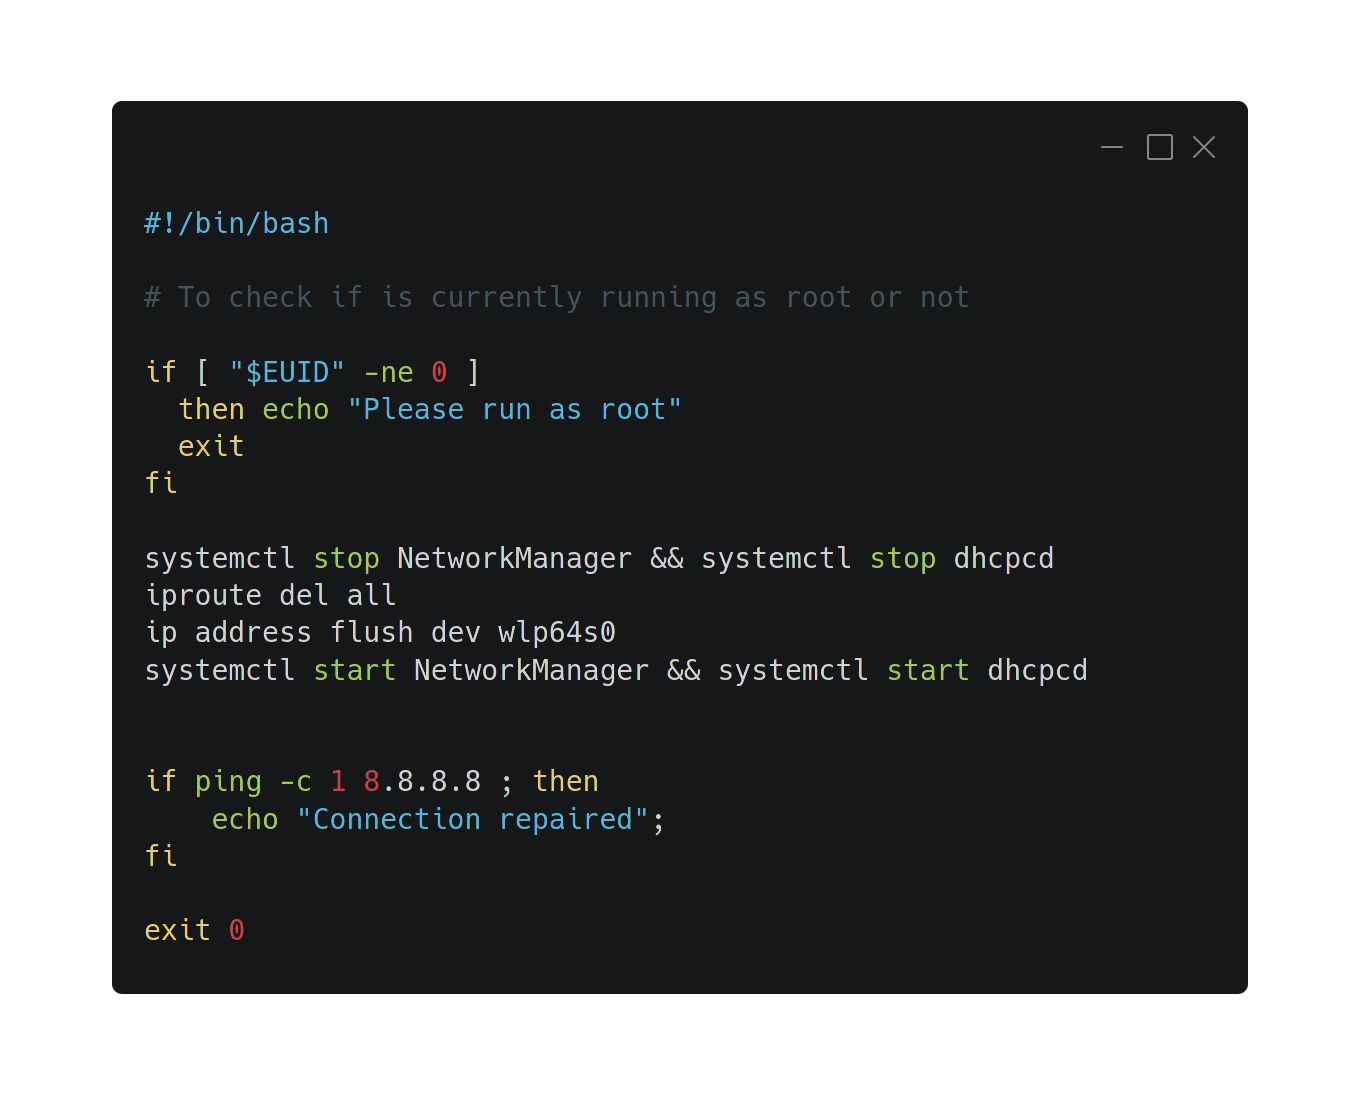
\includegraphics[width=\textwidth]{carbon.png}
% \end{figure}

% Gardez ce bout de code dans un coin, car ça m'a beaucoup aidé pour réparer automatiquement le
% "réseau" sur mon petit OS après qu'un méchant VPN mal configuré ait tout bazardé mes
% configurations.
% \ideaEnd
% On peut aussi afficher du "code" ou tout autre chose d'une façon "bloc note" avec ceci :
% \begin{mycodebox}
%     \begin{verbatim}
%         message :  Q     B     I     T
%         binary : 10000 00001 01000 10011
%         Key :    11100 01011 01001 10010
%         EncrB :  01100 00100 10010 00000
%         EncrM :    M     I     S     A
%     \end{verbatim}
% \end{mycodebox}

% Et si on a \yellowhl{envie} d'inclure directement un fichier \texttt{.txt}, on peut le faire !

% \VerbatimInput{src/contents/quCR_CHSH_Measurement.txt}

% On peut aussi choisir d'écrire directement du code au sein même de notre ligne. Si je veux expliquer que
% \incode{$x = y + 1$}, je peux.

